\documentclass[a4paper,10pt,BCOR=0mm,DIV=14]{scrartcl}

\usepackage[english]{babel}
\usepackage[utf8x]{inputenc}
\usepackage[T1]{fontenc}

\usepackage{csquotes}
\usepackage{graphicx,calc,adjustbox}

\usepackage{hyperref}
\usepackage[noabbrev,english]{cleveref}


\title{Launch of the Entdeckerbox DVD via VirtualBox}

\def\gfxscale{0.27}
\newcommand{\gfxscalebox}[1]{\scalebox{\gfxscale}{#1}}
\newcommand{\smallshadow}[1]{\adjustbox{margin*=-43px -59px -43px  -25px}{#1}}
\newcommand{\command}[1]{\textsf{\enquote{#1}}}

\begin{document}
\maketitle

\section{Introduction}
The Entdeckerbox DVD does not only contain all of the programs, manuals etc., but also provides a live system in order to launch the programs directly, no installation required. For these purposes, the computer needs to be shut down and booted directly from the DVD. 

%Auf der Entdeckerbox-DVD befinden sich nicht nur die einzelnen Programme, Handbücher usw., sondern auch ein Live-System, von dem aus die Programme ohne Installation direkt gestartet werden können. Dazu muss der Computer allerdings heruntergefahren und von der Entdeckerbox-DVD neu gestartet (\enquote{gebootet}) werden.

For security reasons, this is not always possible. In order to use the DVD nonetheless, a virtual machine is needed: A program simulates a complete \enquote{virtual} computer on which the Entdeckerbox live system can be launched. The virtual machine does not have access to the \enquote{real} computer and thus does not pose a security threat. 

%Dies ist -- auch aus Sicherheitsgründen -- nicht überall möglich. Hier bietet eine virtuelle Maschine Abhilfe: Ein Programm simuliert einen vollständigen \enquote{virtuellen} Computer, auf dem das Entdeckerbox-Live-System ausgeführt wird. Sicherheitsbedenkliche Zugriffe auf den \enquote{echten} Computer bleiben der virtuellen Maschine dabei verwehrt.

This document explains how to create such a virtual machine with the open source software Oracle VM VirtualBox. 

%In diesem Dokument wird erklärt, wie man so eine virtuelle Maschine mit der kostenlosen, quelloffenen Software Oracle VM VirtualBox erstellt und verwendet.



\section{Installation of VirtualBox}
The installation files for Oracle VM VirtualBox can be found in the \command{IMAGINARY ENTDECKERBOX} directory of the DVD. Alternatively, you can download the newest version of Oracle VM VirtualBox under \url{https://www.virtualbox.org}. 

%Die Installationsdateien von Oracle VM Virtualbox findest du im \command{IMAGINARY ENTDECKERBOX}-Ordner auf der DVD. Alternativ kannst du auch die jeweils aktuelle Version von Oracle VM VirtualBox auf der Internetseite \url{https://www.virtualbox.org} herunterladen.

Launch the installation program for your operating system and follow the instructions. After launching, your screen should look similar to the one shown in \cref{VBox10}. Please note that there can be slight differences, depending on your operating system. 

%Führe das Installationsprogramm für dein Betriebssystem aus und folge dabei den Anweisungen. Nach dem Start von VirtualBox sollte das Programm etwa wie in \cref{VBox10} aussehen. Bitte beachte, dass sich die folgenden Anweisungen und \nameCrefs{VBox10} je nach Betriebssystem geringfügig unterscheiden können.

\begin{figure}[h!]
\centering \gfxscalebox{\smallshadow{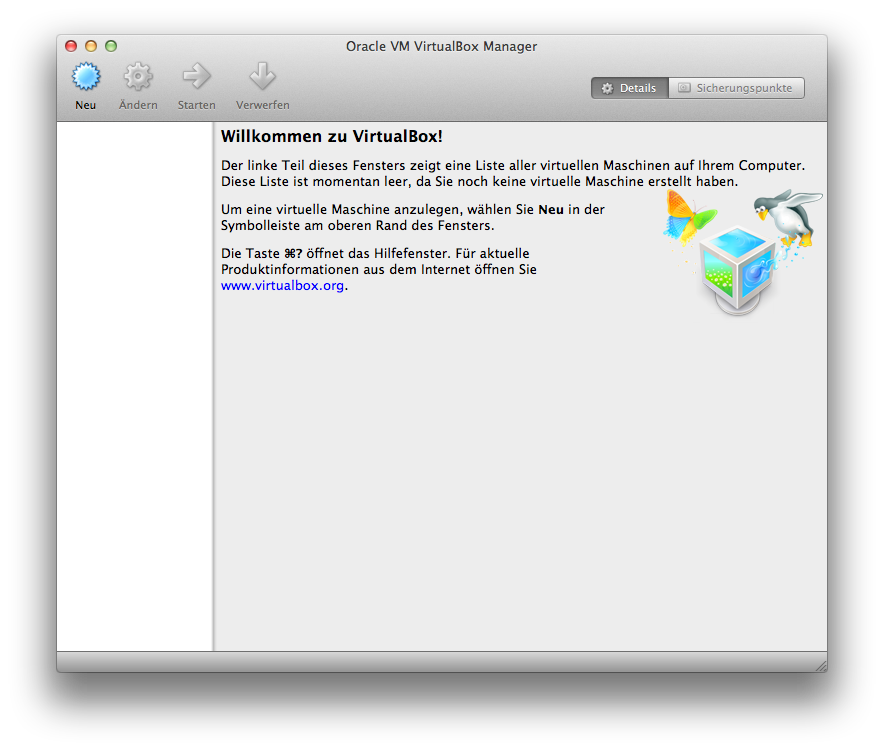
\includegraphics{VBox10}}}
\caption{Start screen of Oracle VM VirtualBox.}
\label{VBox10}
\end{figure}

\section{Create a virtual machine}
In order to create a virtual machine, click on \command{New} in the VirtualBox program. In the following dialogue, you can name your machine, e.\,g. \command{IMAGINARY Entdeckerbox}, and choose type (\command{Linux}) und version (\command{Ubuntu (64\, bit)}) of the system that should run later on. The next step is to choose the size of the internal memory that will be allocated to the virtual machine. The size should not come below 1\, GB, but a bit more doesn't hurt. The next step deals with the creation of a virtual hard drive. Since we want to boot directly from DVD, we can choose \command{Do not add a virtual hard drive} and continue. The newly created virtual machine shows up in the list on the left. This process can be graphically understood in \cref{VBox20to50}. 

%Um nun eine virtuelle Maschine anzulegen, klickt man in VirtualBox of \command{Neu}. Im folgenden Dialog gibt man der virtuellen Maschine einen Namen, z.\,B. \command{IMAGINARY Entdeckerbox} und wählt Typ (\command{Linux}) und Version (\command{Ubuntu (64\, bit)}) des Systems aus, welches später ausgeführt werden soll. Als nächstes stelle man die Größe des Arbeitsspeichers ein, der der virtuellen Maschine zugewiesen werden soll. Hierbei sollte mindestens 1\, GB gewählt werden. Etwas mehr kann aber auch nicht schaden. Der nächste Schritt wäre das Anlegen einer virtuellen Festplatte. Da wir aber von DVD starten wollen, können wir hier \command{Keine Festplatte} auswählen und bestätigen. Jetzt erscheint die frisch erstellte virtuelle Maschine in der Liste auf der linken Seite. Den gesamten Vorgang kannst du noch einmal in \cref{VBox20to50} grafisch nachvollziehen.
\begin{figure}[h]
\centering
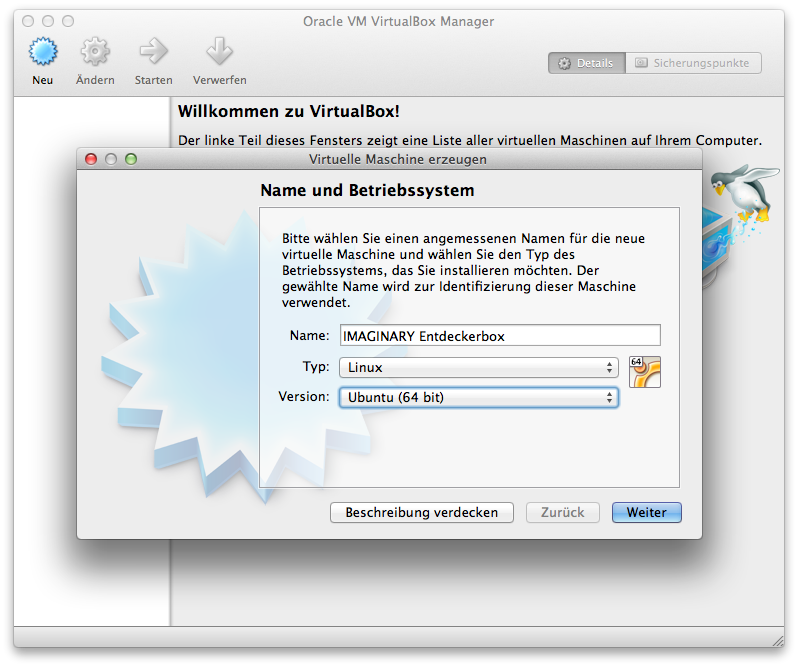
\includegraphics[scale=\gfxscale]{VBox20}
\qquad
\centering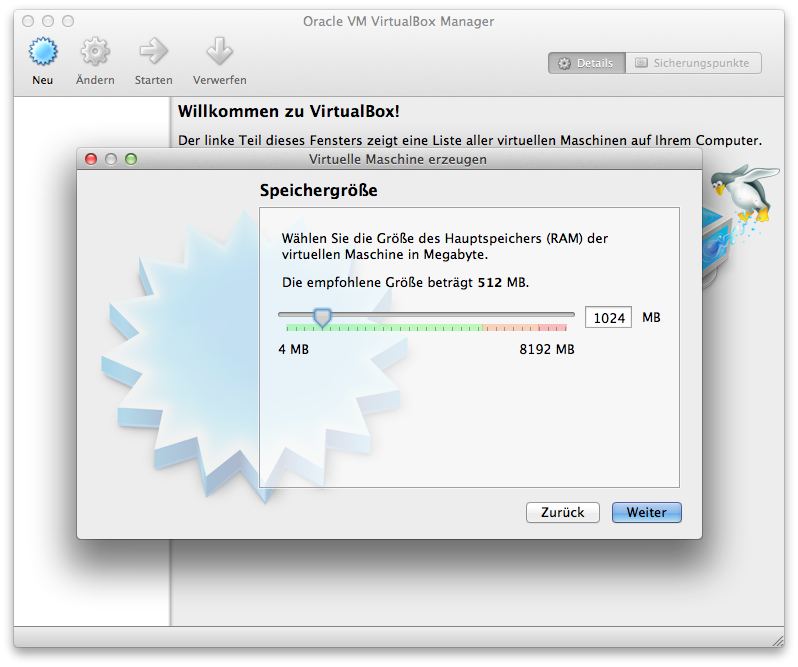
\includegraphics[scale=\gfxscale]{VBox30}
\\[\bigskipamount]
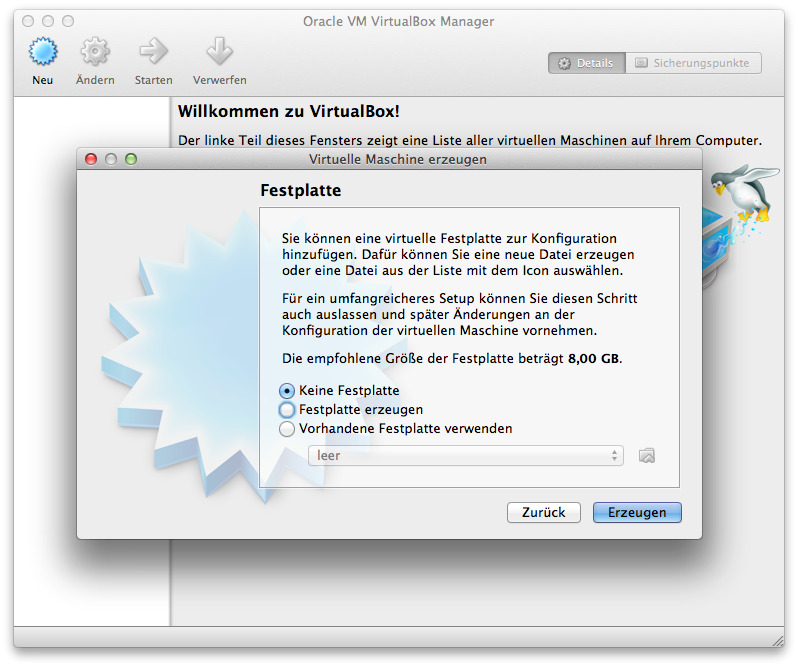
\includegraphics[scale=\gfxscale]{VBox40}
\qquad
\centering\gfxscalebox{\smallshadow{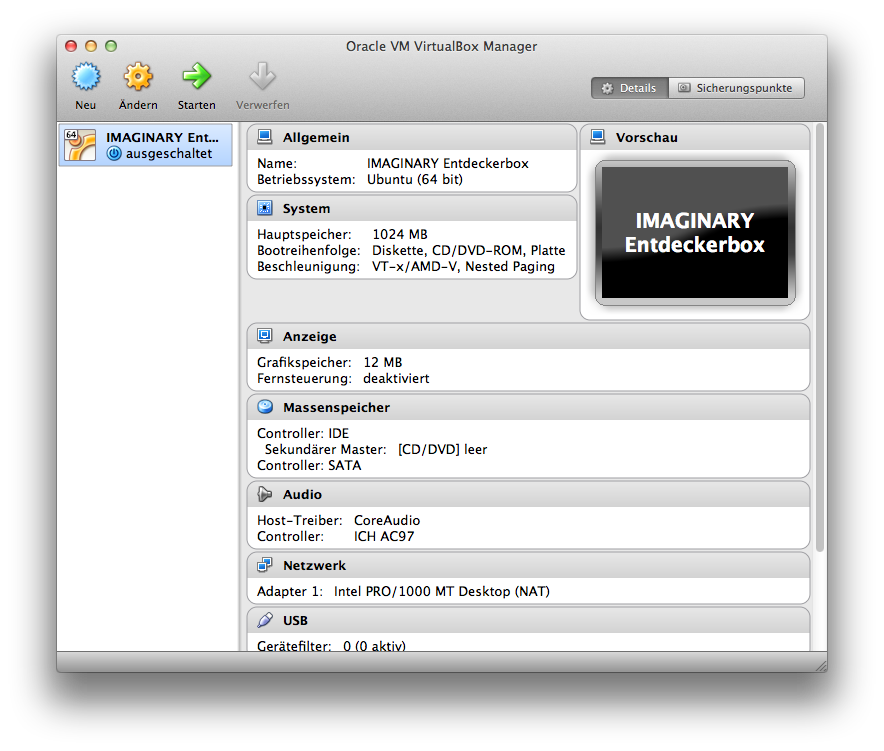
\includegraphics{VBox50}}}
\caption{Steps to create the virtual machine.}
\label{VBox20to50}
\end{figure}

Since some of the programs on the live DVD perform elaborate calculations, it is advisable to allocate more processing power to the virtual machine. For this purpose, choose the machine \command{IMAGINARY Entdeckerbox} from the list and click on \command{Settings}. The menu item \command{System} $\rightarrow$ \command{Processor} lets you choose the number of processors (\command{CPUs}) the virtual machine uses. Within the green range, the number should be as high as possible. In \cref{VBox60}, 8 out of 16 available processors were selected. It is not advisable to choose a number in the red range. If you'd like, you can experiment with the settings in order to obtain the best performance. The video card settings can be found under \command{Display}. You should allocate some graphics memory to the virtual machine and enable the 3d acceleration as shown in \cref{VBox60}. 

%Da einige Programme der Live-DVD sehr aufwendige Berechnungen durchführen, empfiehlt es sich der virtuellen Maschine noch etwas mehr Rechenpower zur Verfügung zu stellen. Wähle hierzu die \command{IMAGINARY Entdeckerbox}-Maschine aus der Liste aus und klicke auf \command{Ändern}. Unter \command{System} $\rightarrow$ \command{Prozessor} kann man festlegen, wie viele Prozessoren (\command{CPUs}) deines Computers die virtuelle Maschine verwenden darf. Innerhalb des grünen Bereichs sollte der Wert hier möglichst hoch eingestellt sein. In \cref{VBox60} wurden also 8 der 16 verfügbaren Prozessoren ausgewählt. Ein Wert innerhalb des roten Bereichs kann in manchen Fällen kontraproduktiv sein. Wer möchte, kann ein wenig mit den Einstellungen experimentieren um die optimale Leistung zu erzielen. Die Einstellungen für die Grafikkarte befinden sich unter \command{Anzeige}. Hier sollte man etwas Grafikspeicher für die virtuelle Maschine reservieren und die 3D-Beschleunigung aktivieren, etwa so wie in \cref{VBox60} gezeigt.
\begin{figure}[h]
\centering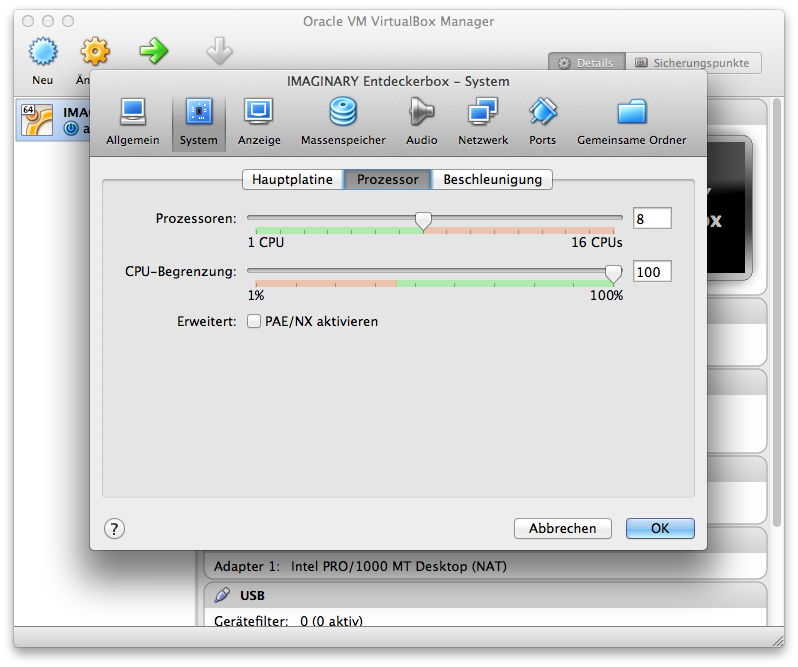
\includegraphics[scale=\gfxscale]{VBox60}
\qquad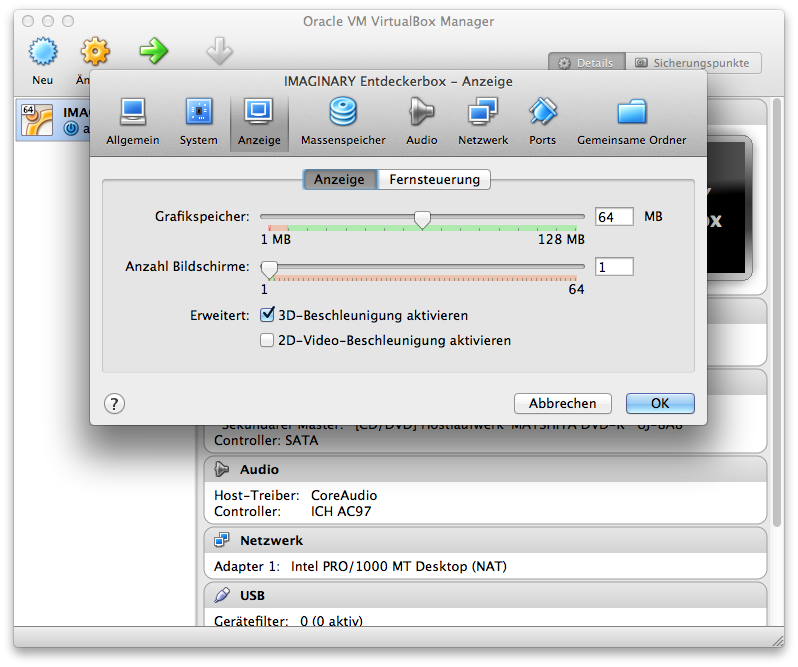
\includegraphics[scale=\gfxscale]{VBox61}
\caption{About half of the available processors should be allocated to the virtual machine. Also, you should increase the graphics memory and enable the 3d acceleration.}
\label{VBox60}
\end{figure}

\section{Launching the Entdeckerbox live DVD}
Before launching the virtual machine, you have to make sure that it actually uses the Entdeckerbox DVD. The virtual DVD drive needs to access the physical DVD drive of your computer. You can change this under \command{Settings} $\rightarrow$ \command{Storage}, as shown in \cref{VBox70}. Please note that the name of your DVD drive showing up behind \command{Host Drive} may be different from the name shown in \cref{VBox70}. Finally, activate the check box \command{Live CD/DVD} and close the dialogue window by clicking on \command{OK}.

%Bevor du die virtuelle Maschine starten kannst, musst du noch sicherstellen, dass dafür auch wirklich die Entdeckerbox-DVD verwendet wird. Das virtuelle DVD-Laufwerk von VirtualBox soll also auf die Entdeckerbox-DVD in dem realen DVD-Laufwerk deines Computers zugreifen. Dies kannst du unter \command{Ändern} $\rightarrow$ \command{Massenspeicher} wie in \cref{VBox70} beschrieben einstellen. Bitte beachte, dass der Name deines DVD-Laufwerks, der hinter \command{Hostlaufwerk} erscheint, wahrscheinlich anders lautet als in der \namecref{VBox70}. Setze nun noch den Haken bei \command{Live-CD/DVD} und beende das Dialogfenster mit \command{OK}.
\begin{figure}[h]
\centering\scalebox{\gfxscale}{\hspace{312px}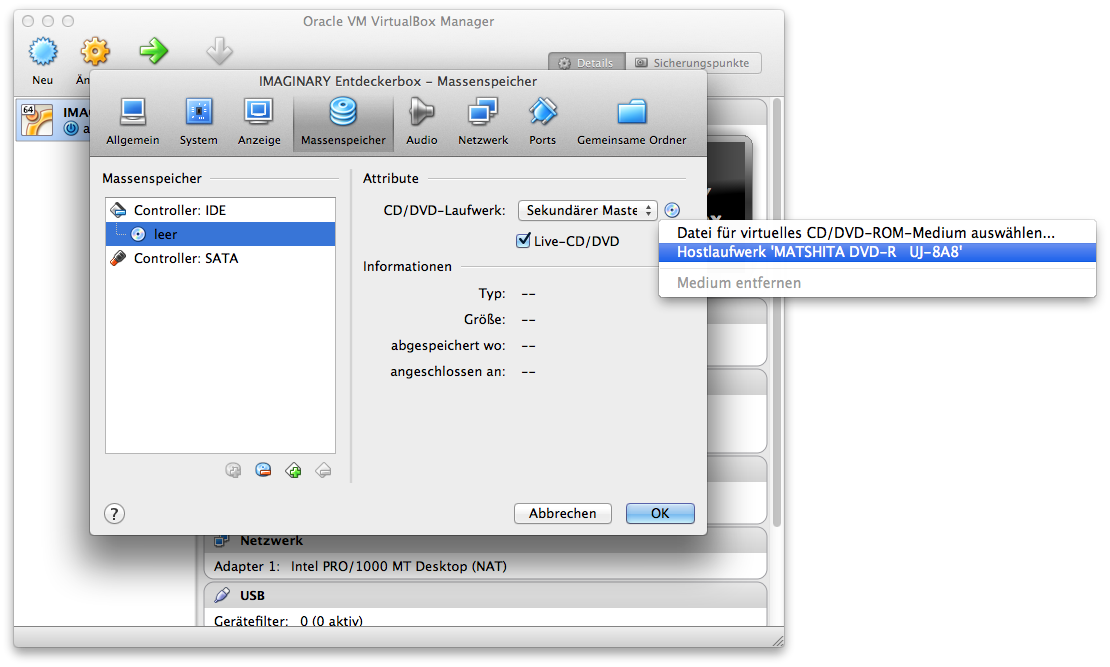
\includegraphics{VBox70}}
\caption{Inserting the Entdeckerbox DVD into the virtual DVD drive.}
\label{VBox70}
\end{figure}

Congratulations! Now everything is set up and you can launch the virtual machine for the first time. By clicking onto the green \command{Start???} arrow, you can boot the system. This should look as in \cref{VBox8090}. 

%Gratulation! Damit sind alle Einstellungen der virtuellen Maschine erledigt und es kann losgehen. Ein Klick auf den grünen \command{Starten}-Pfeil fährt das System hoch. Das sollte etwa so aussehen wie in \cref{VBox8090}.

As you can see, the live DVD runs in window mode. You can change the mode to \command{Full screen} by clicking on \command{View} in the menu of the running virtual machine. Since the programs of the Entdeckerbox DVD do not repsond to these changes in real time, you need to restart them. In the Entdeckerbox menu, for instance, you can change the resoultion by simply hitting \command{ESC}. 

%Wie du siehst, läuft die Live-DVD nun im Fenstermodus. Im Menü der laufenden virtuellen Maschine kann man unter \command{Ansicht} (engl. \command{View}) auf \command{Vollbild} (engl. \command{Fullscreen}) umschalten. Da die Programme auf der Entdeckerbox-DVD nicht automatisch auf diese Umstellung reagieren, müssen sie jeweils neu gestartet werden. Im Entdeckerbox-Menü kann man z.\,B. einfach \command{ESC} drücken. Danach sollte die Auflösung stimmen.

\begin{figure}[h]
\centering
\gfxscalebox{\smallshadow{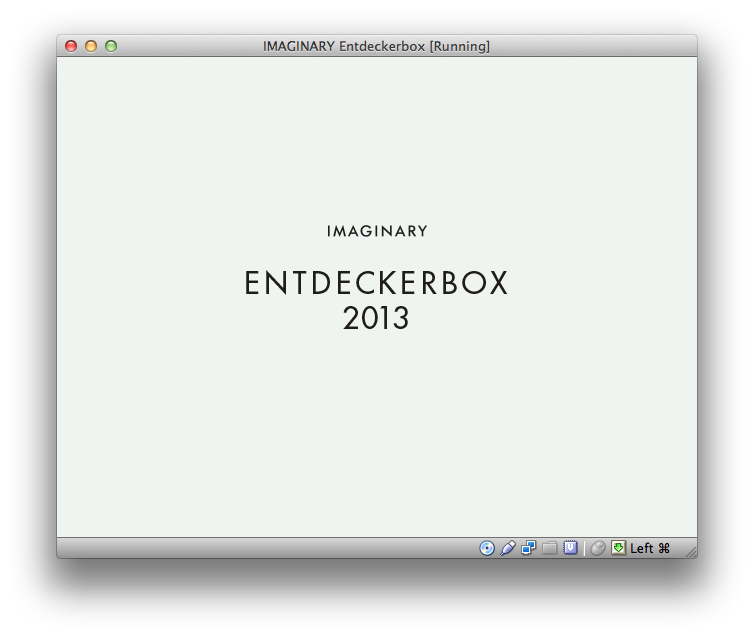
\includegraphics{VBox80}}}
\qquad
\gfxscalebox{\smallshadow{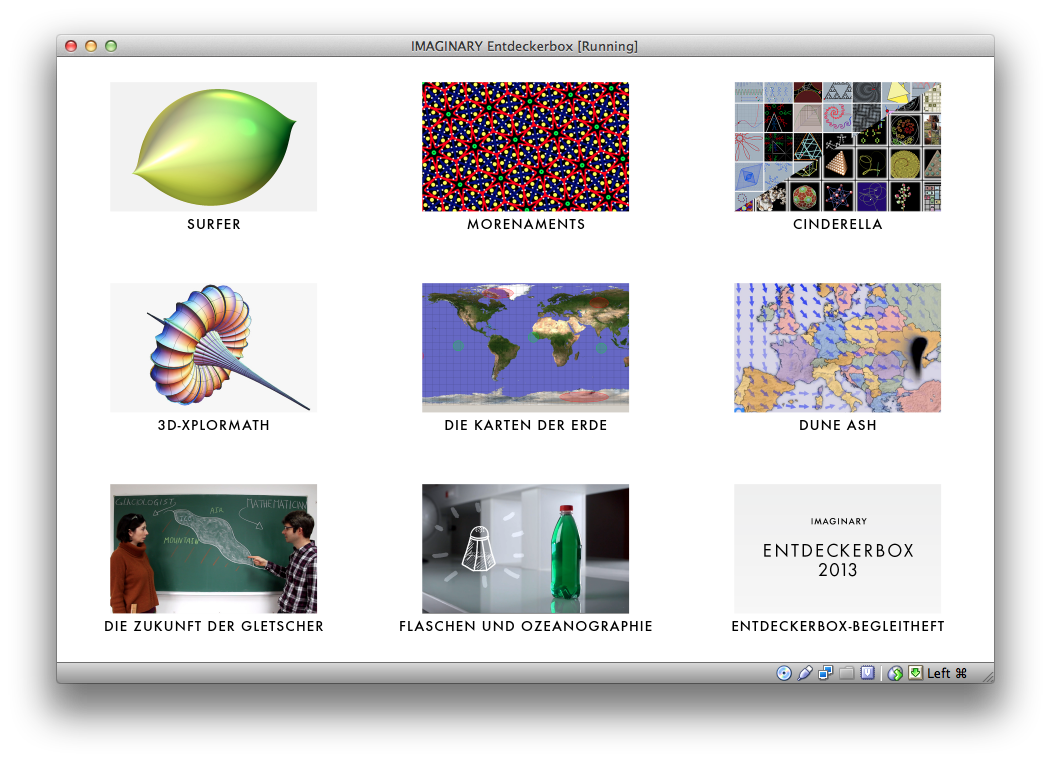
\includegraphics{VBox90}}}
\caption{A while after launching the virtual machine (left), the Entdeckerbox menu shows up (right).}
\label{VBox8090}
\end{figure}

\section{Trouble shooting}
\subsection{I have a 32\,bit operating system, and the live system does not launch!}
Since the live DVD runs with a 64\,bit operating system, a 64\,bit processor is expected. However, VirtualBox can access this from your 32\,bit operating system as long as your processor supports the so-called hardware virtualization. This is the case for pretty much all new processors, although it sometimes needs to be enabled manually in the BIOS. The label of this function differs, depending on the manufacturer (e.\,g. Intel Virtualization Technology, Intel VT-x, Virtualization Extensions, Intel VT-d, AMD-V oder AMD IOMMU). 

%\subsection{Ich habe ein 32\,bit Betriebssystem und das Live-System startet nicht!}
%Auf der Live-DVD befindet sich ein 64\,bit Betriebssystem. Daher wird ein 64\,bit Prozessor vorausgesetzt. VirtualBox kann auch von deinem 32\,bit Betriebssystem darauf zugreifen. Dafür muss dein Prozessor allerdings die sogenannte Hardware-Virtualisierung unterstützen. Dies trifft für die meisten aktuellen Prozessoren zu, jedoch muss diese Funktion manchmal erst im BIOS aktiviert werden. Die Bezeichnung der Funktion ist je nach Hersteller verschieden (z.\,B. Intel Virtualization Technology, Intel VT-x, Virtualization Extensions, Intel VT-d, AMD-V oder AMD IOMMU). 

\subsection{The launch of the live system takes a long time!}
The launch of a complete (albeit virtual) operating system does take some time. It can be drastically reduced though by creating an ISO image of the live system on your hard drive. Depending on the version of the live system (DVD or USB stick), you can find such an ISO image in the same folder as this manual or you have to create it yourself. The required programs are avaiable on the internet for free, for some operating systems they are already included. It is important to create an ISO image on a medium that is noticeably faster than your DVD drive. Solid-state drives are particularly suitable for this purpose. 

%\subsection{Das Starten des Live-Systems dauert lange!}
%Das Starten eines kompletten Betriebssystems von einer DVD dauert leider eine gewisse Zeit. Man kann die Startzeit erheblich reduzieren, indem man ein ISO-Abbild des Live-Systems auf der Festplatte erstellt. Je nach verwendeter Version des Live-Systems (DVD oder USB-Stick) findest du ein solches Abbild im gleichen Dateiordner wie diese Anleitung oder du musst es selbst erstellen. Die dafür benötigten Programme sind im Internet kostenfrei erhältlich. In einigen Betriebssystemen sind sie bereits enthalten. Wichtig ist in jedem Fall, dass das ISO-Abbild auf einem Datenträger abgelegt wird, der deutlich schneller ist als dein DVD-Laufwerk. Besonders geeignet sind hier Solid-State-Disks.

The ISO image should now be inserted into the virtual DVD drive. To this end, click on \command{Choose file for virutal CD/DVD medium???} in the menu shown in \cref{VBox70} and choose the ISO image. 

%Das ISO-Abbild wird nun in das virtuelle DVD-Laufwerk gelegt. Dazu musst du im in \cref{VBox70} gezeigten Menü auf \command{Datei für virtuelles CD/DVD-ROM-Medium auswählen} klicken und das ISO-Abbild auswählen.
\end{document} 
